\documentclass{beamer}
\usetheme{default}
\usepackage[utf8]{inputenc}
\usepackage[spanish]{babel}
\usepackage{hyperref}
\usepackage{wrapfig}
\usetheme{Madrid}
\usecolortheme{seahorse}
\usefonttheme{professionalfonts}
\title{The Computer Scientist as Toolsmith II}
\subtitle{by Fred Brooks}
\author{Antonio, Campos, Chavez, Herrero}
\institute{Ingeniería de Software II}
\date{\today}
\begin{document}

\begin{frame}
\titlepage
\end{frame}

\section{Introduccion}
\begin{frame}{Fred Brooks según Wikipedia}

\begin{itemize}
\item Ingeniero de software y científico de la computación 
\item Ph. D en matemática
\item Fundó el departamento de Computer Science en la Universidad de Carolina del Norte
\item Dirigió el desarrollo del sistema operativo OS/360 de IBM
\item The Mythical Man-Month
\item No Silver Bullet
\item Brooks' law: ``Adding manpower to a late software project makes it later.''
\end{itemize}
\end{frame}

\begin{frame}{Premios}
\begin{itemize}
\item National Medal of Technology - 1985
\item ACM Allen Newell Award - 1994
\item Turing Award - 1999
\end{itemize}
\begin{center}
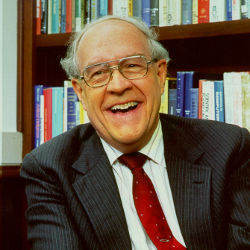
\includegraphics[height=.50\textheight]{Brooks.jpg}
\end{center}
\end{frame}

\begin{frame}{qué significa toolsmith?}
\begin{center}
Persona que hace herramientas
\end{center}
\end{frame}

\begin{frame}{Qué es una ciencia?}
\begin{itemize}
\item Science is a branch of study concerned with the observation and 
classification of facts, especially with the establishment and 
quantitative formulation of verifiable general laws.
\item Científicos construyen para estudiar.
\item Ingenieros estudian para construir.
\end{itemize}
\end{frame}

\begin{frame}{Qué es nuestra disciplina?}
\begin{center}
Ciencias de la computación no es una disciplina científica, 
\newline
es una ingeniería relacionada con crear cosas
\end{center}
\end{frame}

\begin{frame}{Cómo puede un nombre despistarnos?}
\begin{center}
\begin{enumerate}
\item Tendemos a pensar que una ciencia tiene mayor 'valor'
que una ingeniería...
\item Un nuevo hecho, una nueva ley es un logro que
merece publicación.
Si reconocemos nuestros artefactos como herramientas, 
probamos su uso y costo, no por su novedad.
\item Tendemos a olvidar a nuestros usuarios y sus problemas reales,
abstraemos demasiado dejando detrás la esencia del problema real.
\end{enumerate}
\end{center}
\end{frame}

\begin{frame}{La parte Computer está bien}
\begin{itemize}
\item[] La diferencia clave entre ciencas de la computación
y el resto de las ciencias es que somos especialistas en problemas 
que se caracterizan por ser de complejidad arbitraria.
\item[] Matemáticos se escandalizan por la complejidad. 
\item[] Mientras físicos o biólogos se escandalizan por 
la arbitrariedad.
\end{itemize}
\end{frame}

\begin{frame}{Sana evolución de la Inteligencia Artificial}
\begin{itemize}
\item "Haremos máquinas que piensan; haremos Mentes Gigantes"
\item Se ha logrado sorprendentemente poco por el tiempo y la inversión realizada.
\item Estos años de experiencia dieron a los trabajadores en AI 
un respeto profundo por el poder de la mente humana.
\item Es momento de reconocer que los objetivos originales de AI 
no fueron extremadamente difíciles,
fueron objetivos que, aunque glamorosos y motivantes, 
enviaron a la disciplina en una dirección equivocada.
\item En vez de intentar reemplazar la mente humana con máquinas, 
deberíamos estudiar cómo amplificar la mente humana usandolas.
\item Intelligence Amplifying $>$ Artificial Intelligence
\end{itemize}
\end{frame}

\begin{frame}{Colaboración}
\begin{itemize}
\item Debemos asociarnos con aquellos que usarán esas herramientas, aquellos cuya ``inteligencia'' queremos aumentar.
\item Trabajando en los problemas de otras disciplinas, con el fin de colaborar puede, de muchas formas, ayudarnos como computadores científicos.
	\begin{itemize}
	\item Lidiamos con problemas relevantes, y no con ``problemas/ejercicios de juguete''
	\item No nos engañamos con nuestros éxitos o fracasos
	\item Enfrentamos el problema en su totalidad
	\item Y esto nos fuerza a desarrollar áreas que nunca hubieramos investigado
	\item Es divertido (?)
	\end{itemize}
\item En todo trabajo interdisciplinario tiene un costo la ``interacción'': un cuarto del tiempo se va en trabajo inevitable ``de rutina"
\item Idealmente ninguno ``contrata'' a otro
\item Se necesita que los expertos de cada disciplina aprendan sobre la otra
\item El proceso de colaboración de una herramienta debe ser un proceso iterativo para lograr ser exitoso

\end{itemize}
\end{frame}



\end{document}